\documentclass[twocolumn]{IEEEtran}
\usepackage[utf8]{inputenc}
\usepackage{graphicx}
\graphicspath{{figs/}} % No modificar
\usepackage{float}
\usepackage{hyperref}
\usepackage{listings}
\usepackage{xcolor}
\usepackage{multicol}
\lstset{
    basicstyle=\ttfamily\scriptsize,
    breaklines=true,
    breakatwhitespace=false,
    columns=fullflexible,
    frame=single,
    numbers=left,
    numbersep=4pt,
    numberstyle=\tiny,
    xleftmargin=1.5em,
    tabsize=2,
    keywordstyle=\color{blue},
    commentstyle=\color{gray},
    stringstyle=\color{teal}
}
\usepackage[spanish, es-tabla]{babel} % Configura el idioma a español
\addto\captionsspanish{\renewcommand{\abstractname}{Abstract}}

\addto\captionsspanish{\renewcommand{\figurename}{Figura}}
\addto\captionsspanish{\renewcommand{\tablename}{Tabla}}
\usepackage{subcaption}
\usepackage{hyperref}
\hypersetup{
    colorlinks=true,
    linkcolor=blue, % Cambia el color del número si lo deseas
    urlcolor=blue,
}

% \usepackage{ulem}
% http://ctan.org/pkg/{algorithms,algorithmx}
% \usepackage{algorithms,algorithmx}
\renewcommand{\thetable}{\arabic{table}}

\usepackage{hyperref}
\hypersetup{
    colorlinks=true,
    linkcolor=blue,
    filecolor=magenta,      
    urlcolor=blue,
    citecolor = blue,
}
\usepackage{tikz}

\newcommand{\hilight}[1]{\colorbox{yellow}{#1}}
%\numberwithin{equation}{section}
\usepackage{booktabs}
\usepackage{xcolor}
\usepackage{multirow}
\newtheorem{theorem}{Theorem}[section]
\makeatletter
\newcommand{\settheoremtag}[1]{% \settheoremtag{<tag>}
  \let\oldthetheorem\thetheorem% Store \thetheorem
  \renewcommand{\thetheorem}{#1}% Redefine it to a fixed value
  \g@addto@macro\endtheorem{% At \end{theorem}, ...
    \addtocounter{theorem}{-1}% ...restore theorem counter value and...
    \global\let\thetheorem\oldthetheorem}% ...restore \thetheorem
  }
\usepackage{titlesec}

% Cambiar tamaño de las secciones
\titleformat{\section}
  {\normalsize\bfseries}   % tamaño y estilo (large = un poco más grande que normal)
  {\thesection}{1em}  % numeración
  {}

\titleformat{\subsection}
  {\normalsize\bfseries} % tamaño de subsección
  {\thesubsection}{1em}
  {}

% PASO 1. Reemplace "Práctica 1" por el número de la práctica que corresponda
\newcommand{\dochead}{Práctica #2)}     

% PASO 2. Verifique el título de la práctica corresponda.
\newcommand{\docsubhead}{PSD DE SEÑALES ALEATORIAS (GNURADIO)}  

% PASO 3. Reemplace "B1A - 02" por el grupo de la asignatura y el número de su grupo de laboratorio
\newcommand{\teamname}{A1-E}     

% PASO 4. OPCIONAL: Reemplace "\docsubhead \docsubhead" por el título del documento en caso de requerirse.
\newcommand{\titulo}{\dochead: \docsubhead}      

% PASO 5. Reemplace "31 de diciembre de 2030" por la fecha de su documento
\newcommand{\fecha}{Agosto 31, 2026}     

\input{./plantilla.tex}             % No modificar

\usepackage{titlesec}
\titlespacing*{\section}
{0pt}{1ex}{1ex}  % Ajusta el espacio antes y después de las secciones

\usepackage[hidelinks]{hyperref}
\begin{document}  

% No modificar

\title{\vspace{1cm}\textbf{\titulo}}            % No modificar

% PASO 6. Agregar aquí el nombre y código de los autores.  
\author{
Jarol Nicolas Molano Lopez - 2230391 \\
William Camilo Motta Chacon - 2234639\\
Juan Andres Rojas Rueda - 2231065
}
\affil{\small{\url{https://github.com/J202R/2026_2_ComII_A1_A1E}}}
\affil{\normalsize{Escuela de Ingenierías Eléctrica, Electrónica y de Telecomunicaciones} \\ % No modificar
\small{Universidad Industrial de Santander}} % No modificar

\date{\today}

\maketitle                          % No modificar
\thispagestyle{fancy}               % No modificar

%---------------------------------------------------------------
% PASO 7. **..**...****INICIE SU DOCUMENTO DESDE AQUI***...**...
%%%%% A PARTIR DE AQUÍ EDITE EL DOCUMENTO PARA AGREGAR TODO EL CONTENIDO REQUERIDO PARA EL ENTREGABLE CORRESPONDIENTE
%%%%  Todo el contenido a partir de este punto es SOLAMENTE ILUSTRATIVO.
%
% Para sus imformes, BORRE TODO el contenido de aquí en adelante  EXCEPTO la última línea que contiene el comando: \end{document}



% \begin{multicols}{2}
\begin{abstract}
This work computes and interprets the Power Spectral Density (PSD) of a random bipolar rectangular (NRZ) binary signal generated in GNU Radio Companion from the \texttt{randombinayrectsignal.grc} flowgraph. The samples-per-symbol parameter \emph{Sps} was varied (4, 8, 16, and 1) with a fixed sampling frequency $f_s=128$ kHz, in order to observe its effect on the time-domain waveform and on the PSD, and to compare the observed null positions with the theoretical bit rate $R_b$ and bandwidth $BW$. The binary signal was also compared against Gaussian white noise, and the spectral occupancy was evaluated when the bits originate from real information sources (an image, \texttt{rana.jpg}, and an audio file, \texttt{sonido.wav}) instead of an independent random source. Results show that the $\text{sinc}^2$ envelope is preserved in all cases, while the internal correlation of real data introduces additional discrete spectral components that are absent in the purely random case.
\end{abstract}


\begin{IEEEkeywords}
GNU Radio, Power Spectral Density, random binary signal, NRZ, white noise
\end{IEEEkeywords}


\section{Introducción}

La Densidad Espectral de Potencia (PSD) describe cómo se distribuye la energía de una señal en función de la frecuencia, revelando información que no es evidente en el dominio del tiempo, tal como el ancho de banda ocupado, la forma de los lóbulos espectrales y el efecto que tiene la codificación de línea o el tipo de fuente de información sobre la ocupación espectral. En esta práctica se calcula e interpreta la PSD de una señal binaria aleatoria bipolar de forma rectangular utilizando \textbf{GNU Radio Companion}, a partir del flujograma \texttt{randombinayrectsignal.grc}. Se varía el parámetro \emph{Sps} (muestras por símbolo) para observar su efecto en el dominio del tiempo y en la PSD, se compara el comportamiento espectral de la señal binaria frente al de ruido blanco, y se evalúa cómo cambia la ocupación espectral cuando los bits provienen de fuentes reales de información: una imagen (\texttt{rana.jpg}) y un archivo de audio (\texttt{sonido.wav}). El objetivo es interiorizar los conceptos de señales aleatorias necesarios para calcular e interpretar correctamente su PSD.





\section{Metodología}

\subsection{Fundamento teórico}
Para una señal binaria bipolar de forma rectangular (NRZ), la PSD teórica corresponde a la función $\text{sinc}^2(f \, T_b)$, donde $T_b = 1/R_b$ es la duración de un símbolo y $R_b$ la tasa de bits \cite{ortega2019comunicaciones}. Esta forma presenta un lóbulo principal cuyo primer nulo ocurre en $f = R_b$, por lo que el ancho de banda de primer nulo se define como $BW = 2R_b$, y lóbulos secundarios decrecientes espaciados también en $R_b$. En el flujograma, cada símbolo se repite \emph{Sps} veces mediante el bloque \emph{Interpolation FIR Filter}, de modo que la tasa de bits queda determinada por la frecuencia de muestreo $f_s$ y el factor de interpolación como $R_b = f_s / Sps$. Esta relación explica por qué, al aumentar \emph{Sps}, disminuye $R_b$ y con ello se angosta el lóbulo principal de la PSD; repetir cada símbolo \emph{Sps} veces es, en esencia, un filtrado tipo promedio móvil (\emph{moving average}) de longitud \emph{Sps}, cuyo ancho de banda es inversamente proporcional a dicha longitud \cite{wavewalkerdsp2022ma}. La estimación de la PSD en GNU Radio se realiza mediante un periodograma (promedio de $|\text{FFT}|^2$ de bloques sucesivos de la señal) \cite{tijaro2025timeaverages}, lo cual introduce un piso de resolución espectral dependiente del tamaño de la FFT y de $f_s$, aspecto relevante al interpretar los lóbulos observados frente a los valores teóricos.

\subsection{Configuración del flujograma base}
Se utilizó el flujograma \texttt{randombinayrectsignal.grc} \cite{ortega2021grc}, el cual genera una señal binaria aleatoria a partir de un bloque \emph{Random Source} seguido de \emph{Unpack K Bits} y \emph{Char to Float}. La conversión de la señal unipolar (0/1) a bipolar ($-1$/$1$) se realiza con una combinación de bloques \emph{Constant Source}, \emph{Add} y \emph{Multiply Const}. Finalmente, un bloque \emph{Interpolation FIR Filter}, configurado con factor de interpolación igual a \emph{Sps}, repite cada símbolo el número de muestras correspondiente, fijando así la relación entre $R_b$, $f_s$ y \emph{Sps} descrita en la sección anterior.

\subsection{Variación del parámetro Sps}
Sobre el flujograma base se varió el vector de taps \emph{h} del \emph{Interpolation FIR Filter} para que \emph{Sps} tomara los valores $4$, $8$, $16$ y $1$, manteniendo $f_s = 128$ kHz. Para cada valor se registró la forma en el tiempo de la señal en el punto p4 y su PSD, y se contrastaron contra los parámetros de transmisión teóricos ($R_b$, $f_s$ y $BW$, calculados con las expresiones de la sección anterior y resumidos en la Tabla~\ref{tab:sps} de la sección de Resultados), verificando que la posición de los nulos observados en cada PSD correspondiera con el $BW$ teórico esperado.

\subsection{Comportamiento del ruido blanco}
Se configuraron los bloques \emph{Virtual Source} de los puntos de prueba p4 y p5 para comparar, en tiempo y en PSD, la señal binaria bipolar frente a una fuente de ruido blanco, con el fin de contrastar el ancho de banda observado en GNU Radio con el concepto teórico de ancho de banda infinito del ruido blanco \cite{ortega2019comunicaciones}.

\subsection{Señal a partir de una fuente real: imagen}
Se reemplazó el bloque \emph{Random Source} por la combinación \emph{File Source} + \emph{Unpack K Bits}, configurando el parámetro \texttt{File} para leer \texttt{rana.jpg} \cite{ortega2021rana}. De esta forma los bits dejaron de ser estadísticamente independientes y pasaron a representar la información real de la imagen, lo que permite analizar el efecto de la estructura del archivo sobre la PSD resultante.

\subsection{Señal a partir de una fuente real: audio}
Siguiendo el mismo procedimiento del numeral anterior, se configuró el bloque \emph{File Source} para leer \texttt{sonido.wav} \cite{ortega2021sonido}, manteniendo el mismo factor de interpolación ($Sps=4$) usado en la primera prueba de la Tabla~\ref{tab:sps}, con el fin de evaluar el efecto de una fuente de audio real sobre la forma temporal y la PSD de la señal binaria generada, y de comparar dicho comportamiento tanto con el caso de la imagen como con los parámetros teóricos ($R_b=32$ kHz, $BW=64$ kHz) obtenidos en la Tabla~\ref{tab:sps}.


























\section{Resultados y Análisis de Datos}

Para todos los casos se utilizó el flujograma \texttt{randombinayrectsignal.grc} \cite{ortega2021grc} (Figura~\ref{fig:instrumentacion}), con una frecuencia de muestreo fija $f_s = 128$ kHz. Al variar el vector \emph{h} (taps del \emph{Interpolation FIR Filter}) se modificaba el parámetro \emph{Sps}, lo que a su vez determinaba la tasa de bits mediante $R_b = f_s / Sps$. Repetir cada símbolo \emph{Sps} veces equivalía, en frecuencia, a un filtro promediador (\emph{moving average}) de longitud \emph{Sps}, cuyo ancho de banda decrecía al aumentar el número de muestras promediadas \cite{wavewalkerdsp2022ma}.

\begin{figure}[h]
    \centering
    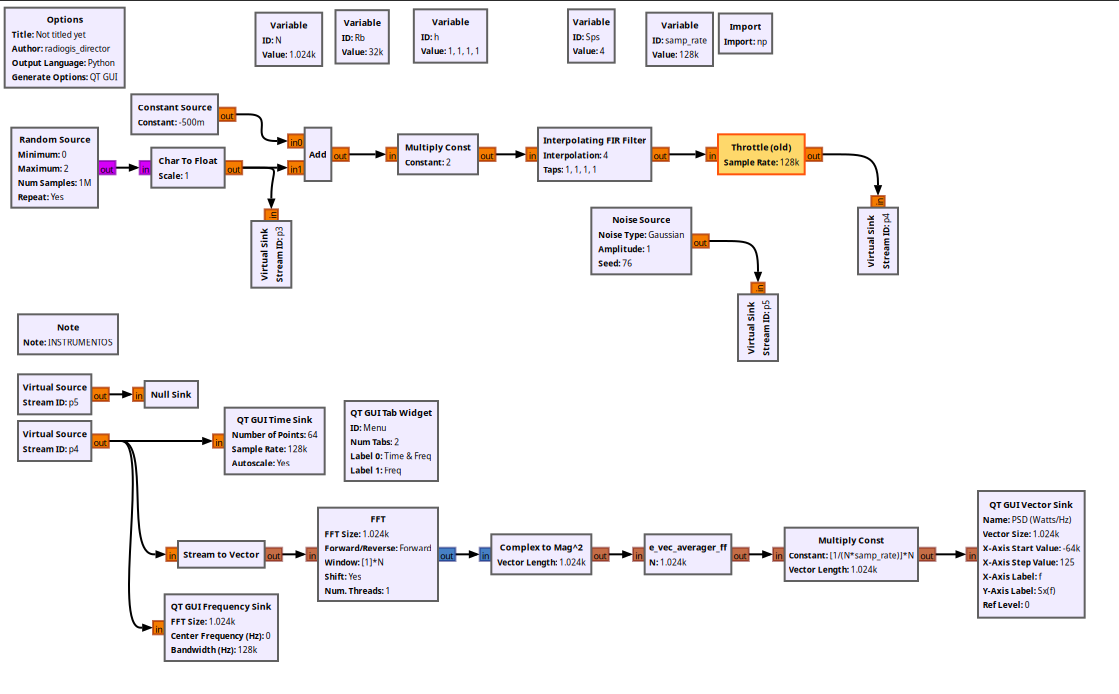
\includegraphics[width=0.85\linewidth]{1788670098664_image.png}
    \\[1.5em]
    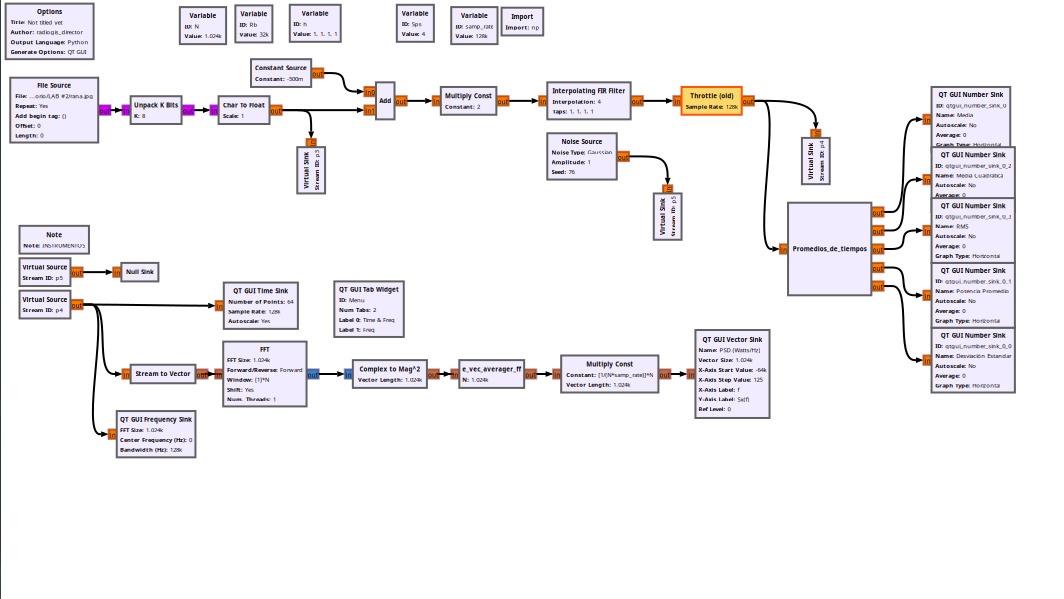
\includegraphics[width=0.85\linewidth]{flujograma_con_bloque_estadistico.png}
    \caption{\textbf{Imagen Superior}: Flujograma original utilizado \cite{ortega2021grc}: generación de la señal binaria bipolar (p3), inyección de ruido blanco (p5) y cadena de instrumentación para el cálculo de la PSD sobre p4. 
    \textbf{Imagen Inferior}: Mismo flujograma con la modificación del bloque estadístico de promedios de tiempo.}
    \label{fig:instrumentacion}
\end{figure}

\subsection{Efecto del parámetro Sps sobre la señal binaria bipolar}

La Tabla~\ref{tab:sps} resume, a partir de $R_b = f_s/Sps$ y del ancho de banda de primer nulo $BW = 2R_b$, los parámetros teóricos esperados para cada configuración \cite{ortega2019comunicaciones}.

\begin{table}[h]
\centering
\caption{Parámetros teóricos de la señal binaria bipolar para $f_s = 128$ kHz}
\label{tab:sps}
\begin{tabular}{cccc}
\hline
\textbf{Sps} & \textbf{$R_b$ (kHz)} & \textbf{$f_s$ (kHz)} & \textbf{BW teórico (kHz)} \\
\hline
4  & 32  & 128 & 64  \\
8  & 16  & 128 & 32  \\
16 & 8   & 128 & 16  \\
1  & 128 & 128 & 256 \\
\hline
\end{tabular}
\end{table}

\begin{figure}[h]
    \centering
    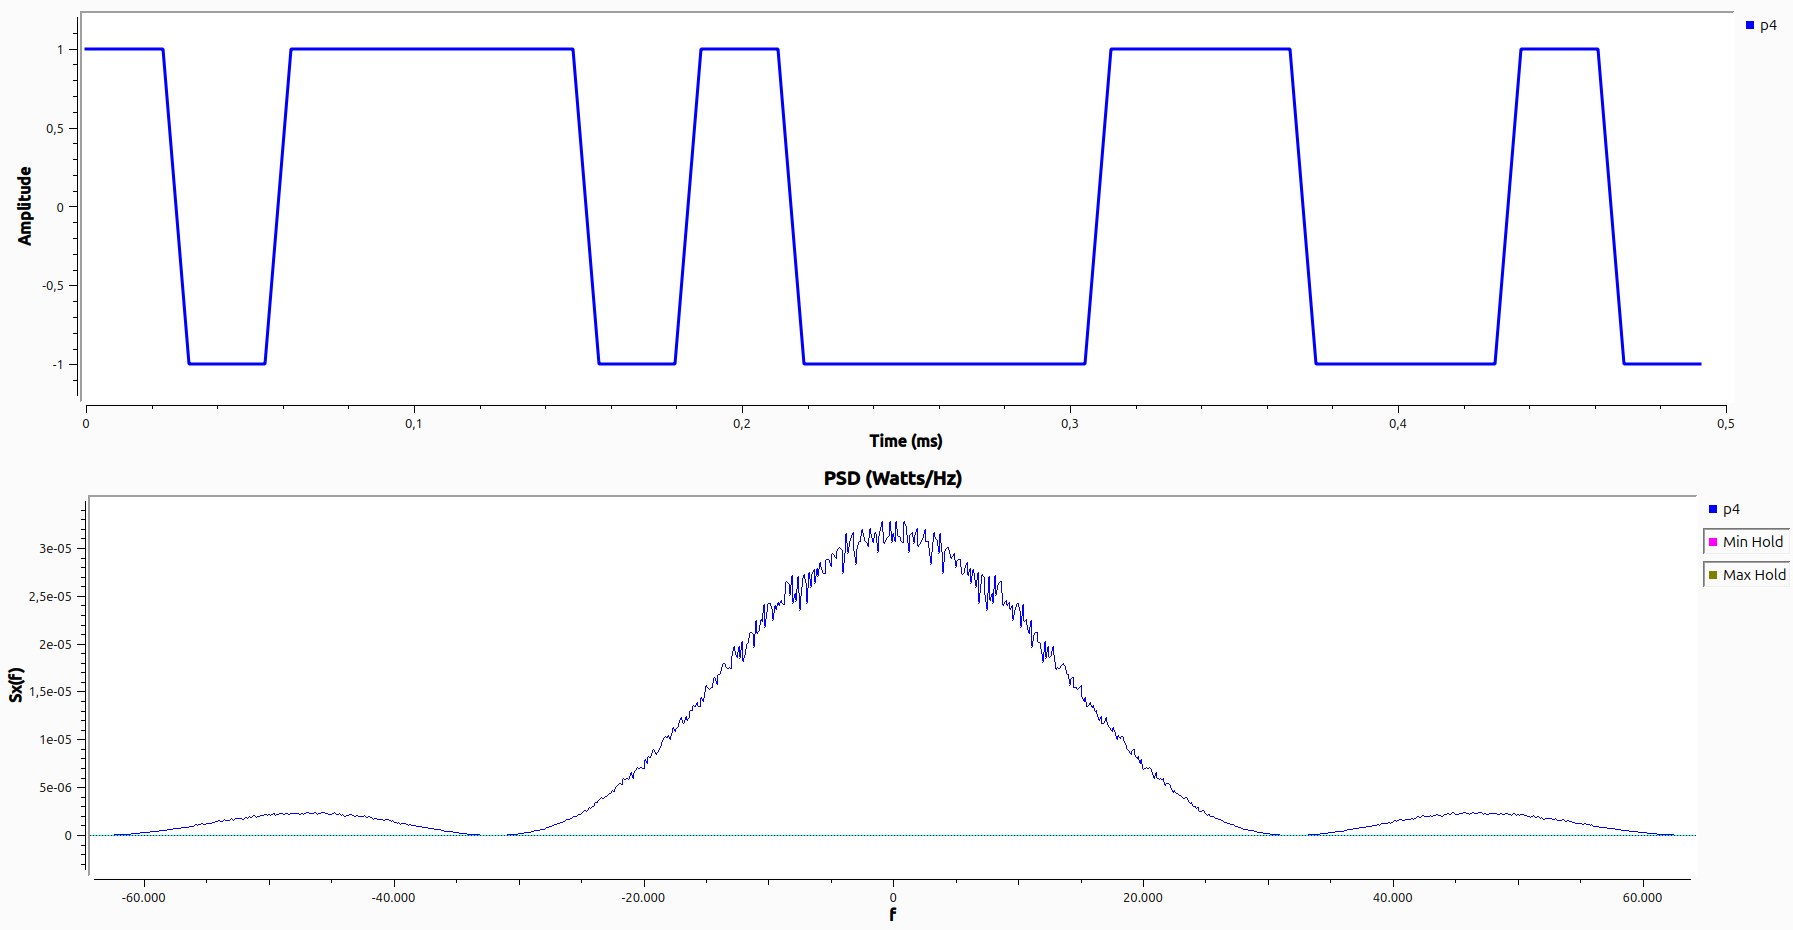
\includegraphics[width=0.7\linewidth]{1788669972941_image.png}
    \caption{Resultados para $Sps=4$: forma en el tiempo y PSD (Watts/Hz) de la señal en p4.}
    \label{fig:sps4}
\end{figure}

Como se observó en la Figura~\ref{fig:sps4}, en el panel superior la señal en el tiempo alternó limpiamente entre $-1$ y $+1$ con flancos casi verticales, mostrando alrededor de cinco pulsos completos en la ventana de $0$ a $0.5$~ms. En el panel inferior, la PSD (escala lineal, eje de frecuencia $\pm 60$~kHz) presentó un lóbulo principal centrado en $f=0$ con su primer nulo próximo a $R_b=32$ kHz, seguido de dos lóbulos secundarios decrecientes visibles cerca de $\pm 45$–$50$ kHz, en concordancia con la forma $\text{sinc}^2$ esperada para un pulso rectangular bipolar. Esta figura no incluyó panel en dB.

\begin{figure}[h]
    \centering
    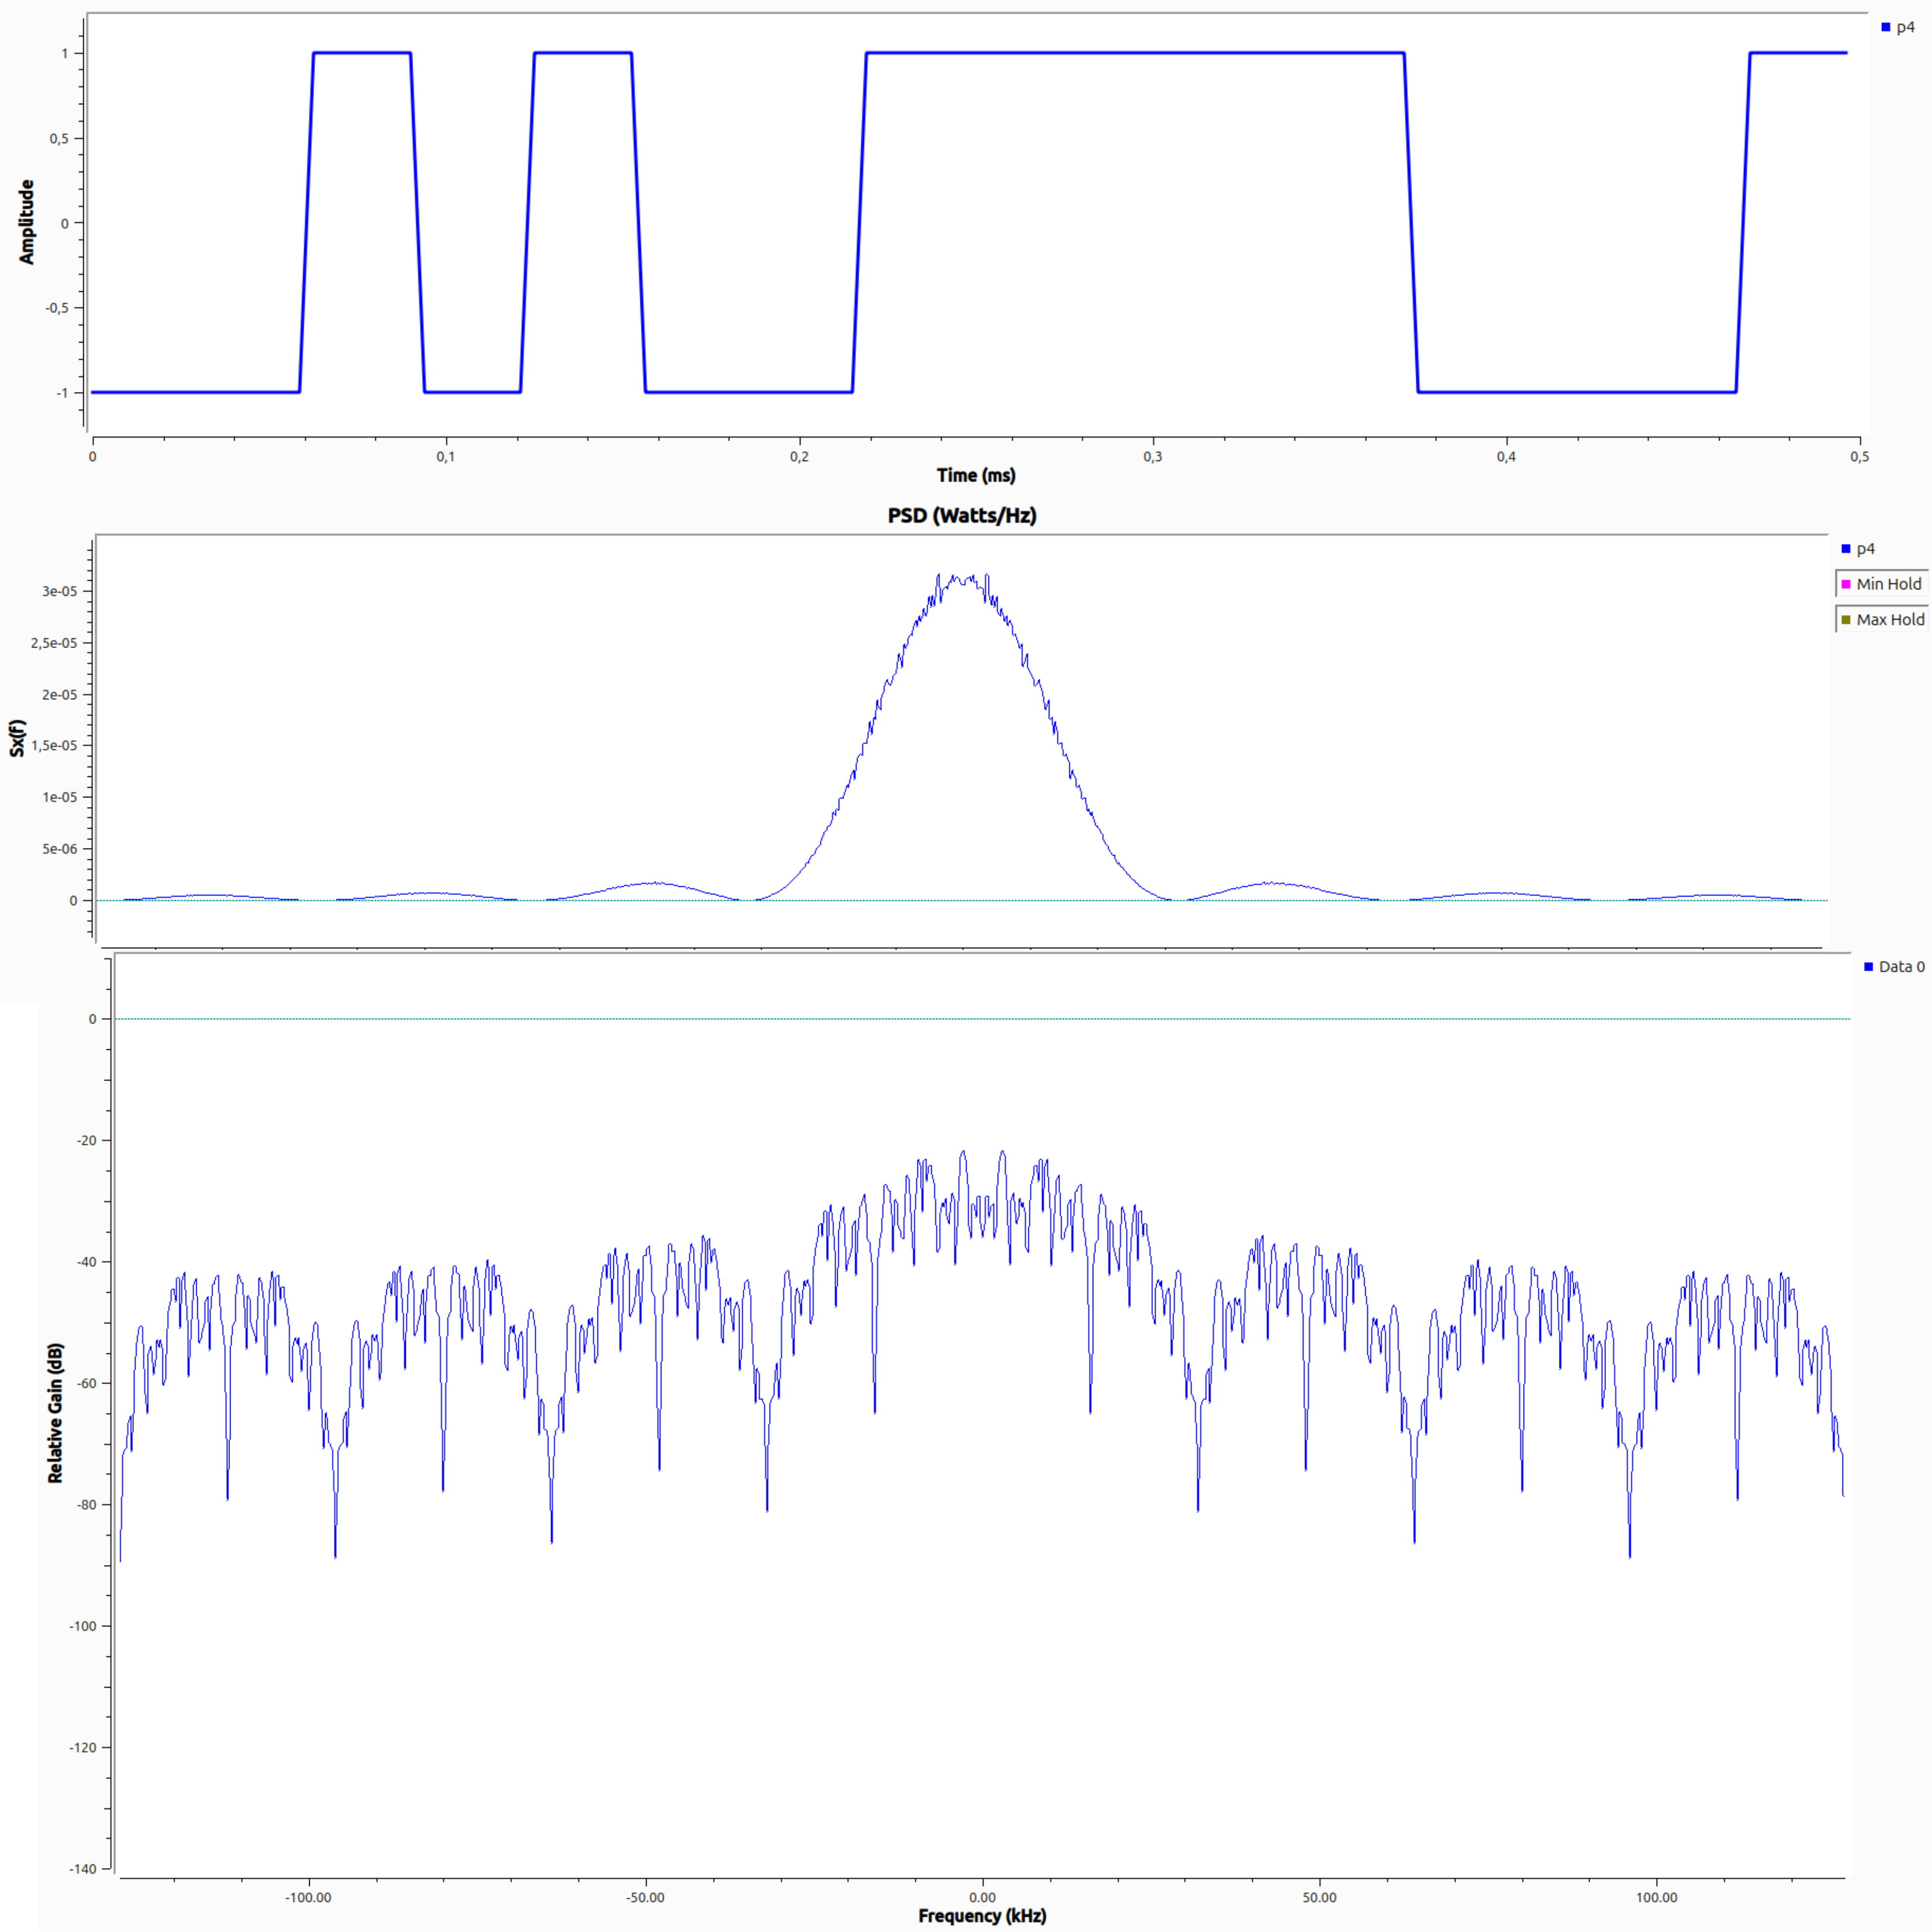
\includegraphics[width=0.6\linewidth]{1788670000711_image.png}
    \caption{Resultados para $Sps=8$. \textbf{Arriba}: tiempo y PSD (Watts/Hz). \textbf{Abajo}: PSD en dB.}
    \label{fig:sps8}
\end{figure}

Al duplicar \emph{Sps}, $R_b$ se redujo a la mitad (16 kHz), lo que angostó el lóbulo principal de la PSD respecto al caso anterior (Figura~\ref{fig:sps8}), confirmando la relación inversa entre el ancho temporal del símbolo y el ancho de banda ocupado. En el dominio del tiempo se observaron pulsos de duración irregular (propio de la aleatoriedad de los símbolos), con menos transiciones que en la Figura~\ref{fig:sps4}. El panel inferior (dB) mostró la envolvente $\text{sinc}^2$ cubierta por el rizado característico del promedio de periodogramas sucesivos \cite{tijaro2025timeaverages}, con lóbulos secundarios espaciados de forma aproximadamente regular.

%CORRECCIÓN: el eje de frecuencia del panel dB de esta figura llega a aprox. $\pm100$ kHz, mientras que el de la Figura~\ref{fig:sps4} llega solo a $\pm60$ kHz. Como $f_s=128$ kHz es fija en todos los casos, se recomienda fijar el mismo rango de frecuencia en todas las figuras de PSD para que el "angostamiento" del lóbulo sea comparable visualmente y no un efecto del zoom del eje.

\begin{figure}[h]
    \centering
    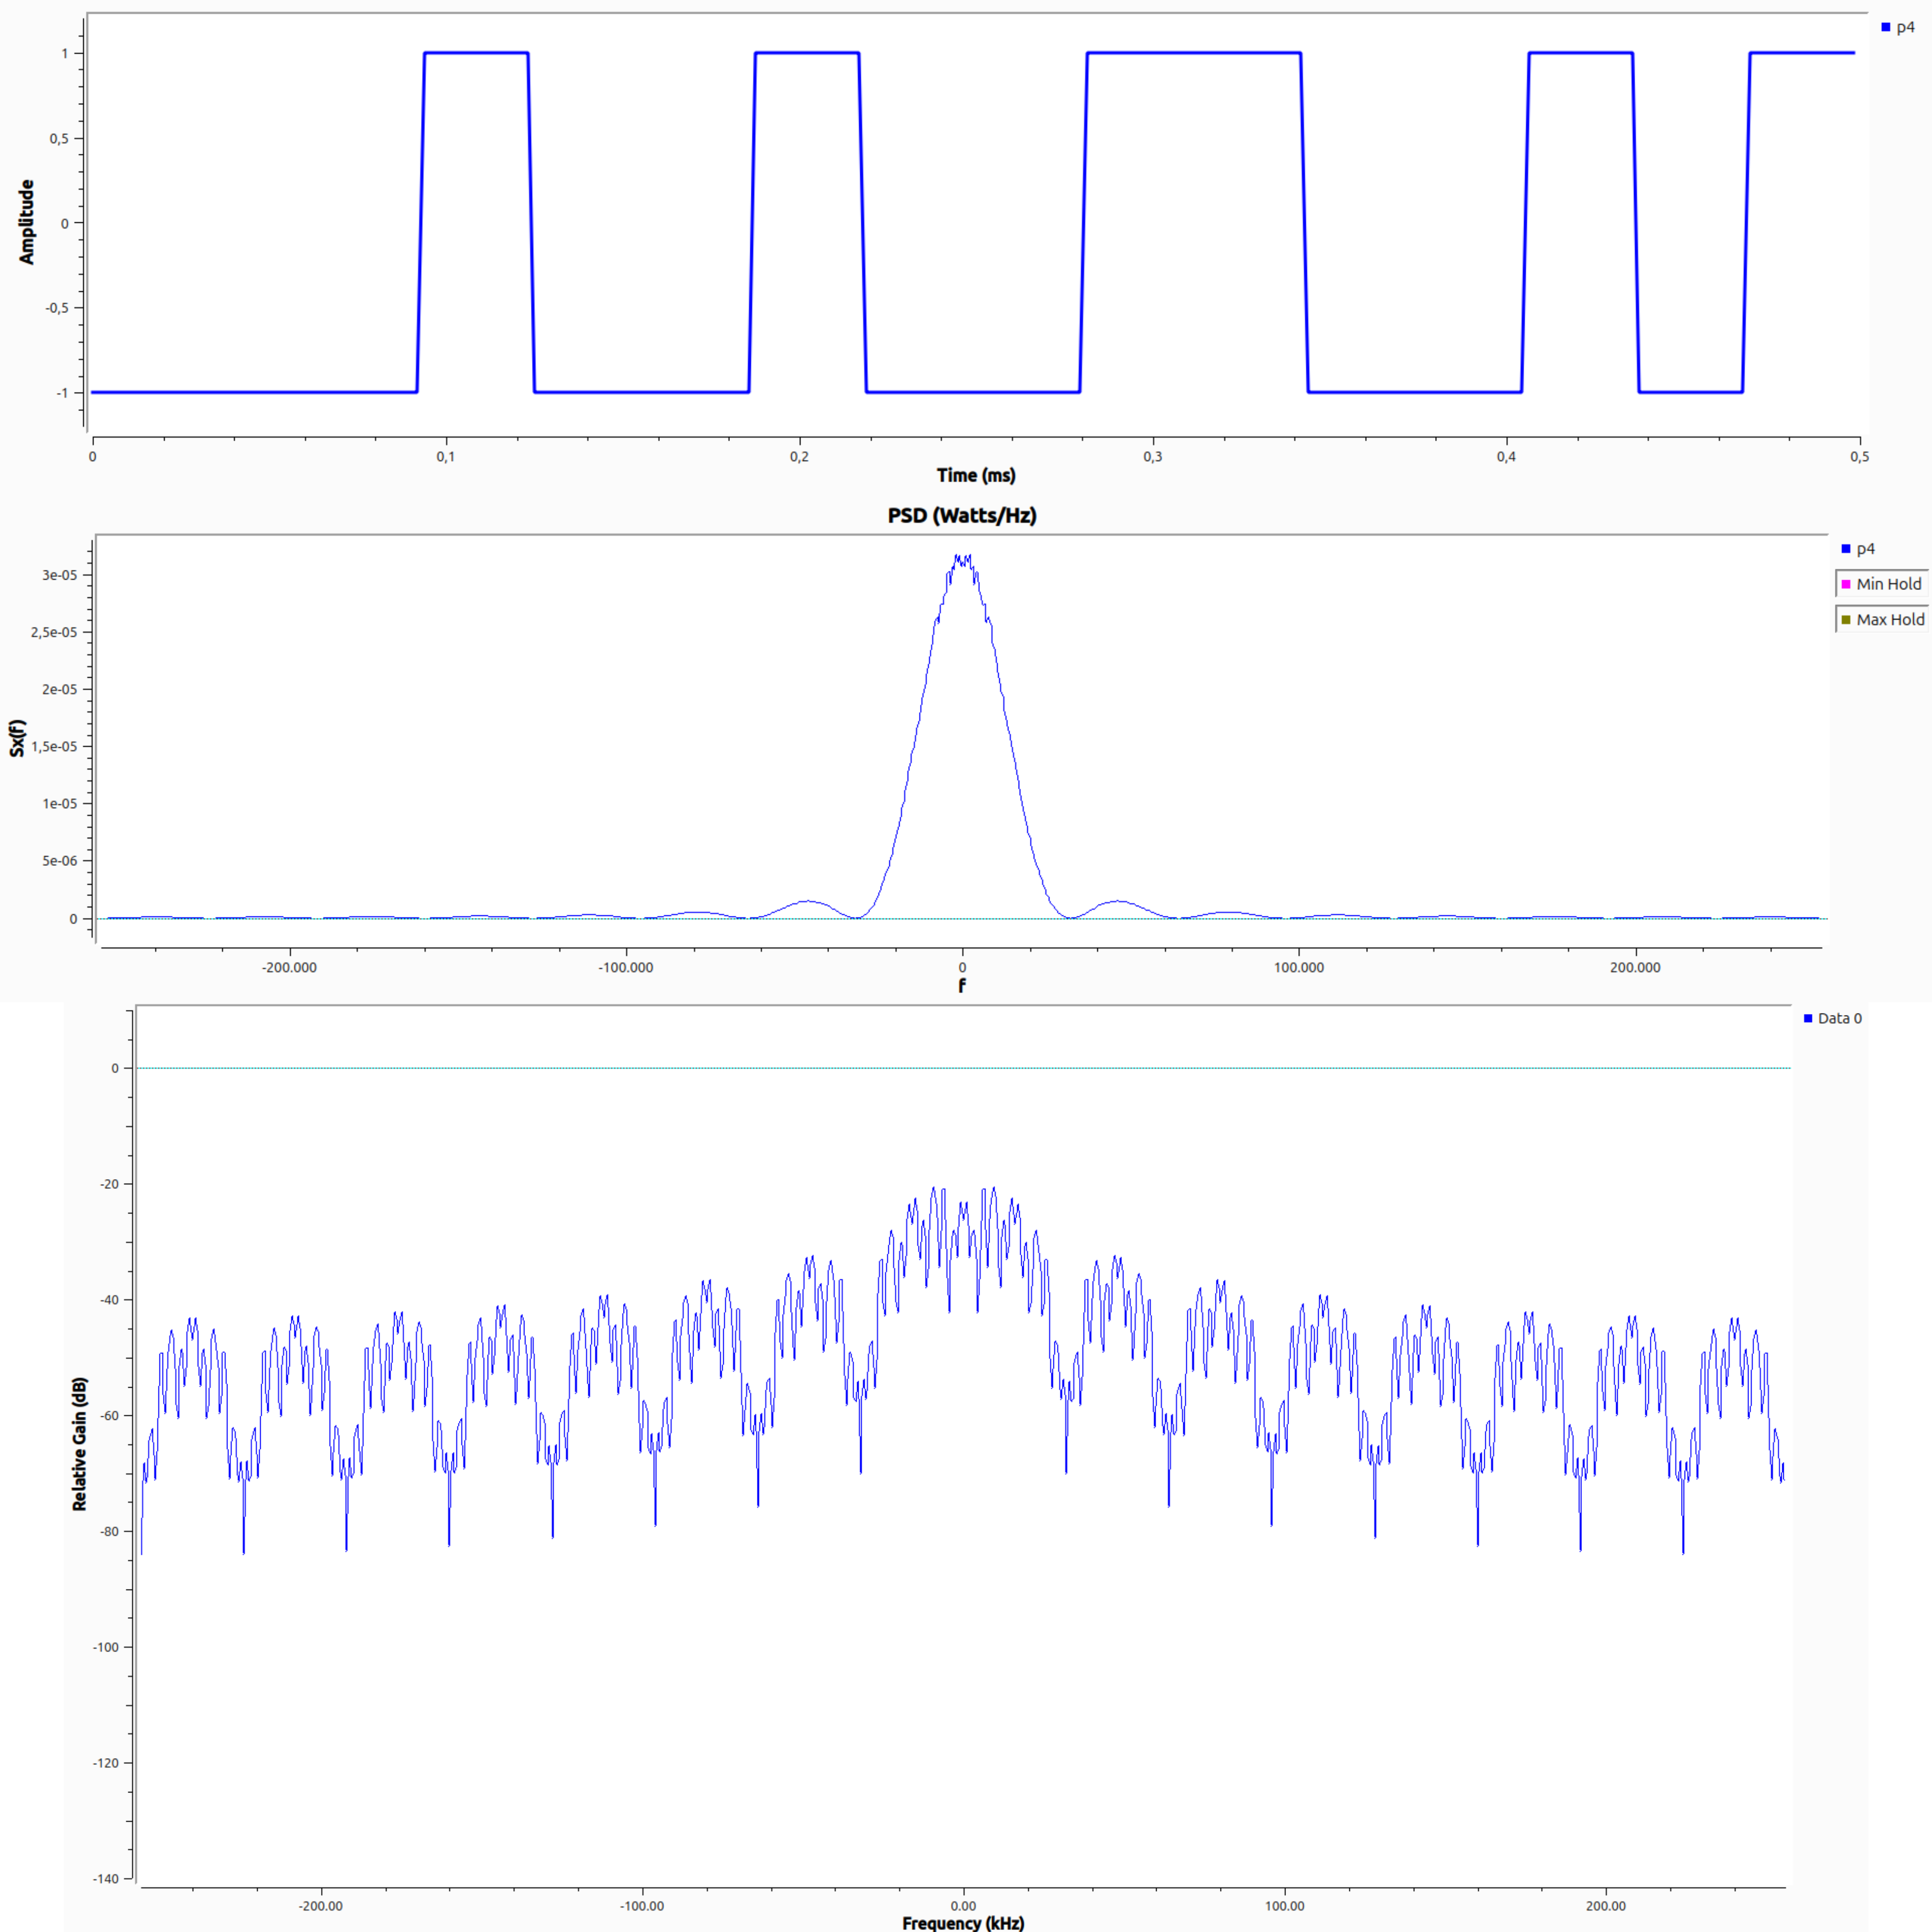
\includegraphics[width=0.6\7\linewidth]{1788670019375_image.png}
    \caption{Resultados para $Sps=16$. \textbf{Arriba}: tiempo y PSD (Watts/Hz). \textbf{Abajo}: PSD en dB.}
    \label{fig:sps16}
\end{figure}

Para $Sps=16$ (Figura~\ref{fig:sps16}), $R_b$ bajó a 8 kHz y el lóbulo principal se angostó aún más, lo que confirmó que a mayor número de muestras por símbolo, menor era el ancho de banda ocupado, a costa de una menor tasa de transmisión efectiva.

%CORRECCIÓN: el eje de frecuencia del panel superior (lineal) de esta figura se extiende hasta aprox. $\pm 200$–$256$ kHz. Esto excede el límite de Nyquist $f_s/2 = 64$ kHz que ustedes mismos citan en la Sección~\ref{ref_ruido} para $f_s=128$ kHz fija; revisar la configuración del \emph{QT GUI Frequency Sink}/rango de eje usado para esta captura antes de publicar, porque no debería ser posible observar contenido espectral fuera de $[-64,64]$ kHz.

\begin{figure}[h]
    \centering
    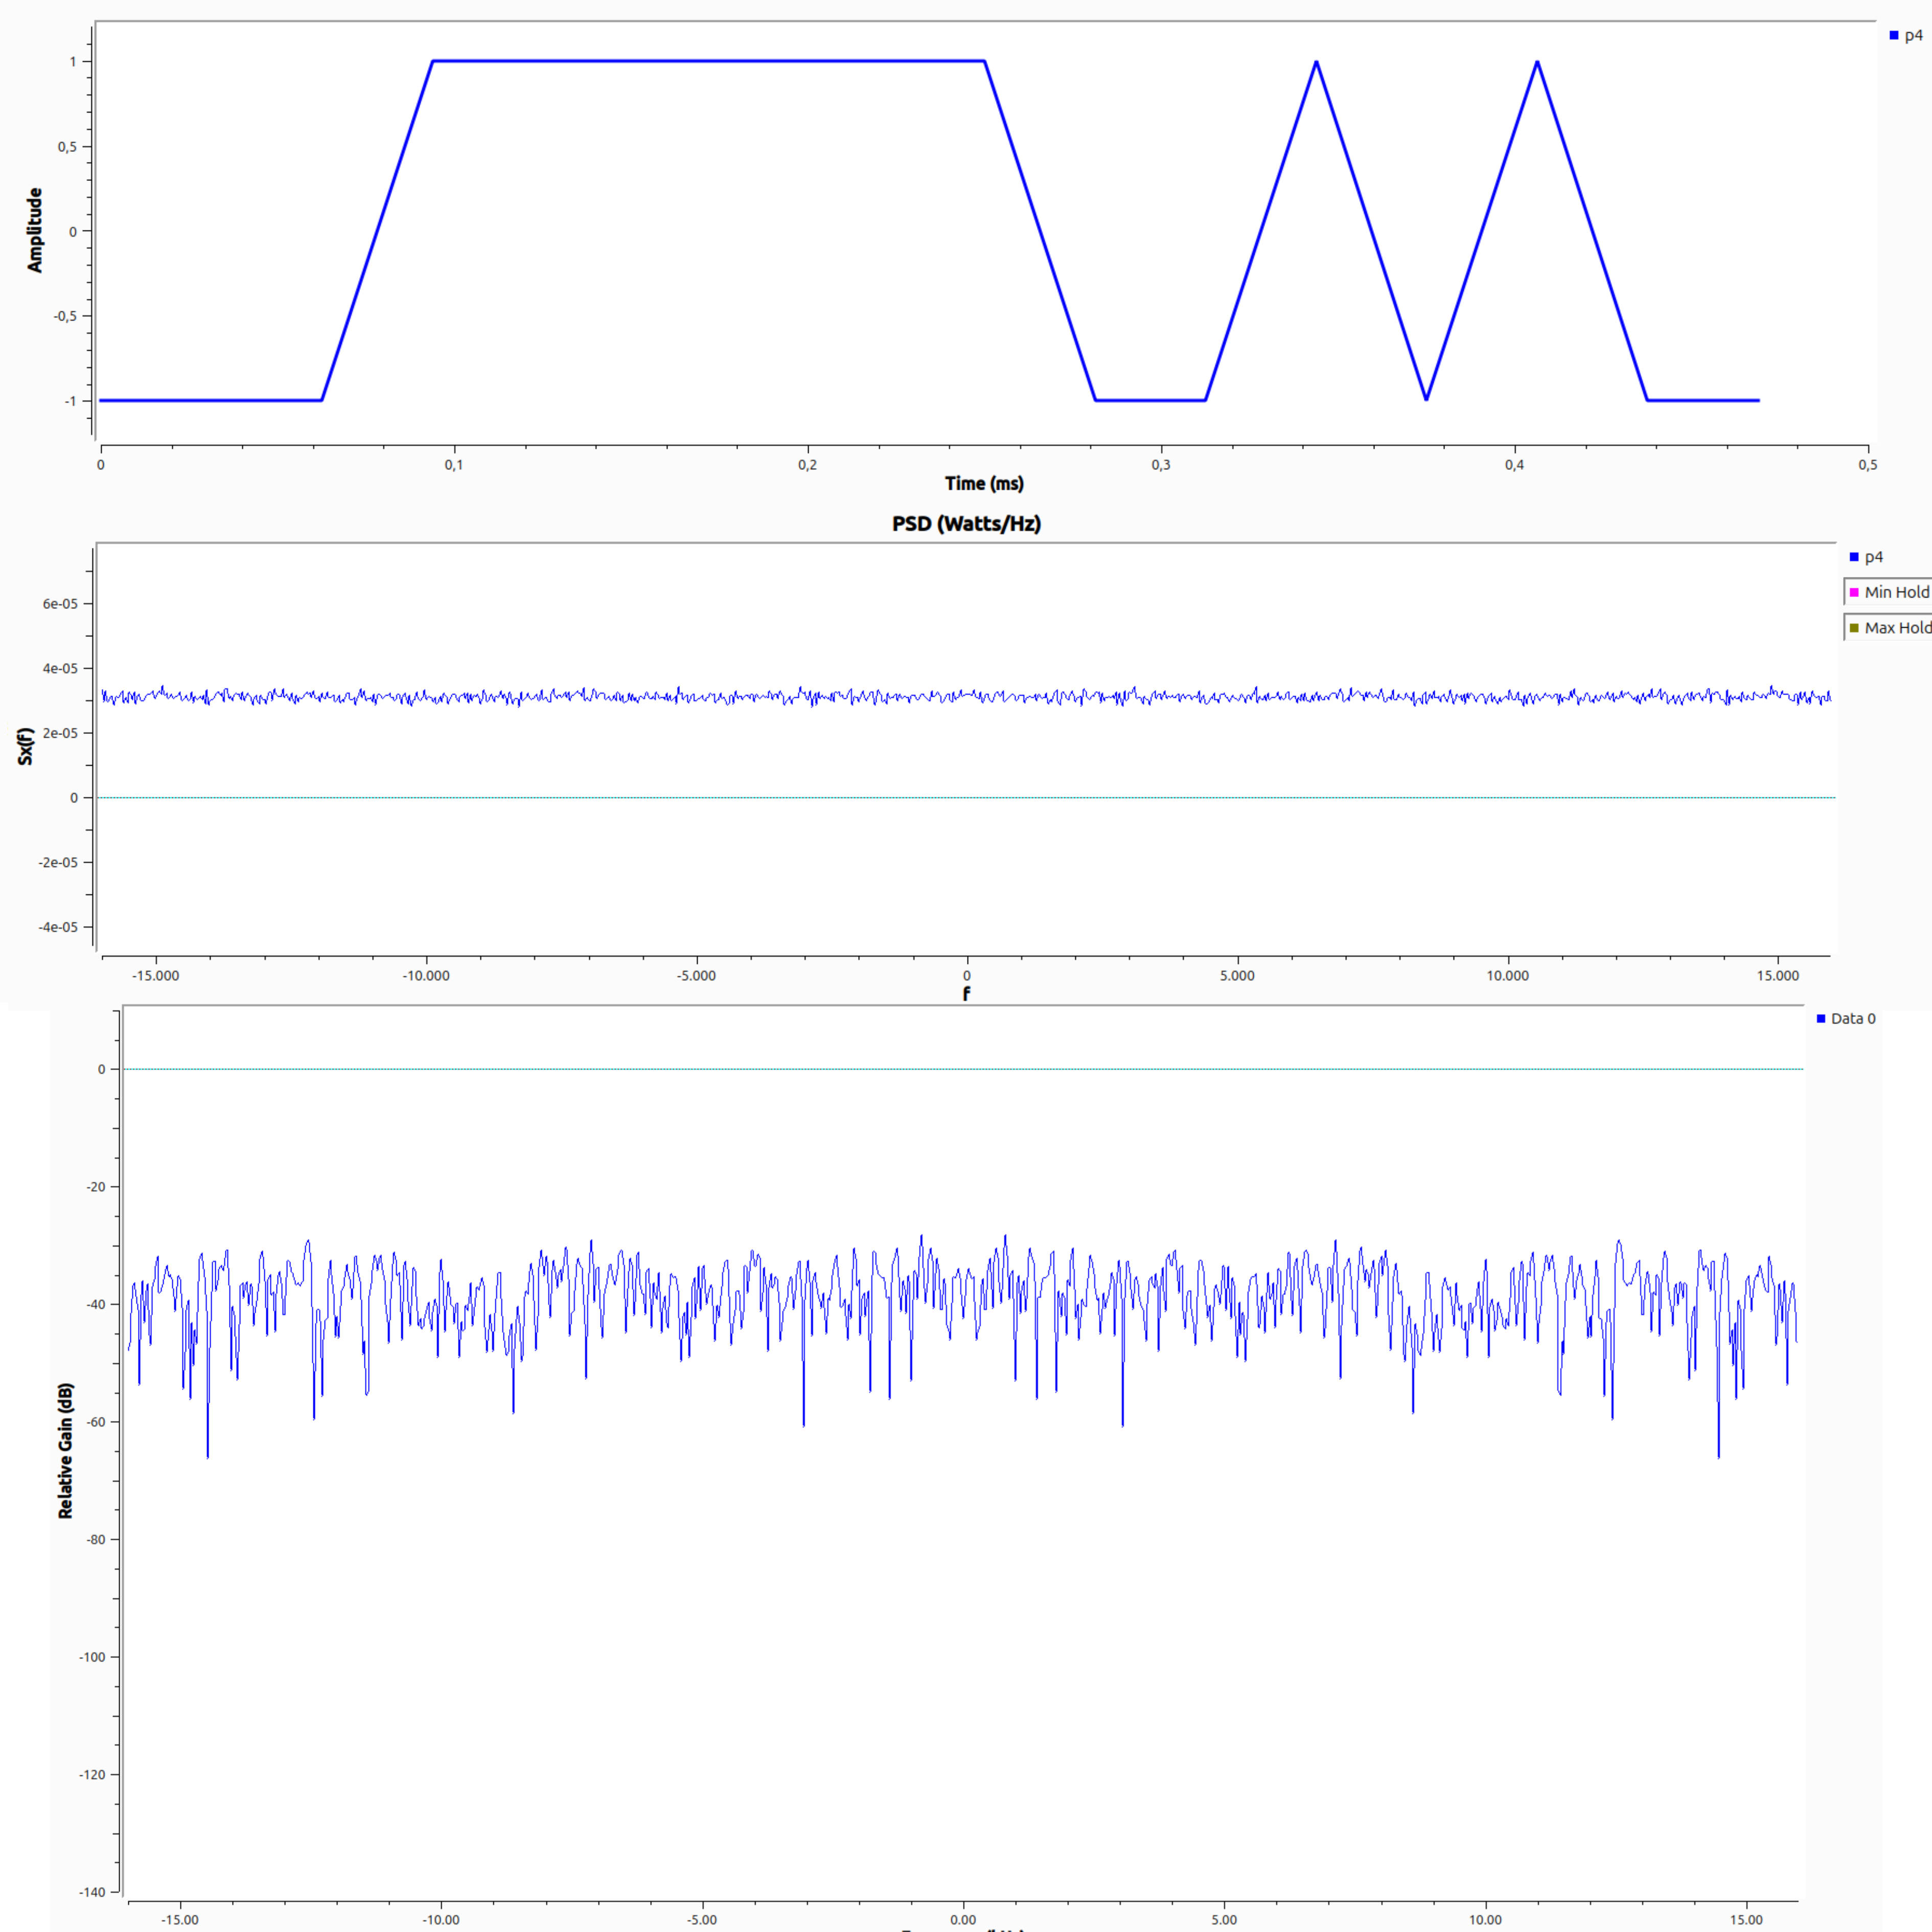
\includegraphics[width=0.6\linewidth]{1788669986860_image.png}
    \caption{Resultados para $Sps=1$. \textbf{Arriba}: tiempo y PSD (Watts/Hz). \textbf{Abajo}: PSD en dB.}
    \label{fig:sps1}
\end{figure}

El caso $Sps=1$ (Figura~\ref{fig:sps1}) correspondió al extremo opuesto: $R_b=f_s=128$ kHz, por lo que la PSD se percibió prácticamente plana dentro de la ventana de observación (eje $\pm15$ kHz, tanto en escala lineal como en dB), ya que su ancho de banda teórico (256 kHz) excedía ampliamente el rango mostrado.

%CORRECCIÓN: el panel superior (tiempo) de esta figura no muestra lo que cabría esperar para $Sps=1$. En vez de una secuencia de saltos abruptos entre $-1$ y $+1$ (un valor independiente por muestra), se observan solo 4-5 transiciones en la ventana de 0.5~ms, unidas por \emph{rampas suaves} que tardan del orden de $50\ \mu\text{s}$ en pasar de $-1$ a $+1$ (unas 6-7 muestras a $f_s=128$ kHz). Con $T_b \approx 7.8\ \mu\text{s}$, en esa ventana deberían verse decenas de transiciones independientes, no una forma tipo rampa/triángulo. Esto contradice directamente la afirmación de que "no hay suavizado entre símbolos": lo que se ve es, si acaso, más suavizado que en los casos $Sps=4,8,16$. Se recomienda revisar el vector de taps \emph{h} configurado para $Sps=1$ en el \emph{Interpolation FIR Filter} antes de dar esta captura por válida.

\subsection{Comportamiento del ruido blanco}
\label{ref_ruido}

\begin{figure}[h]
    \centering
    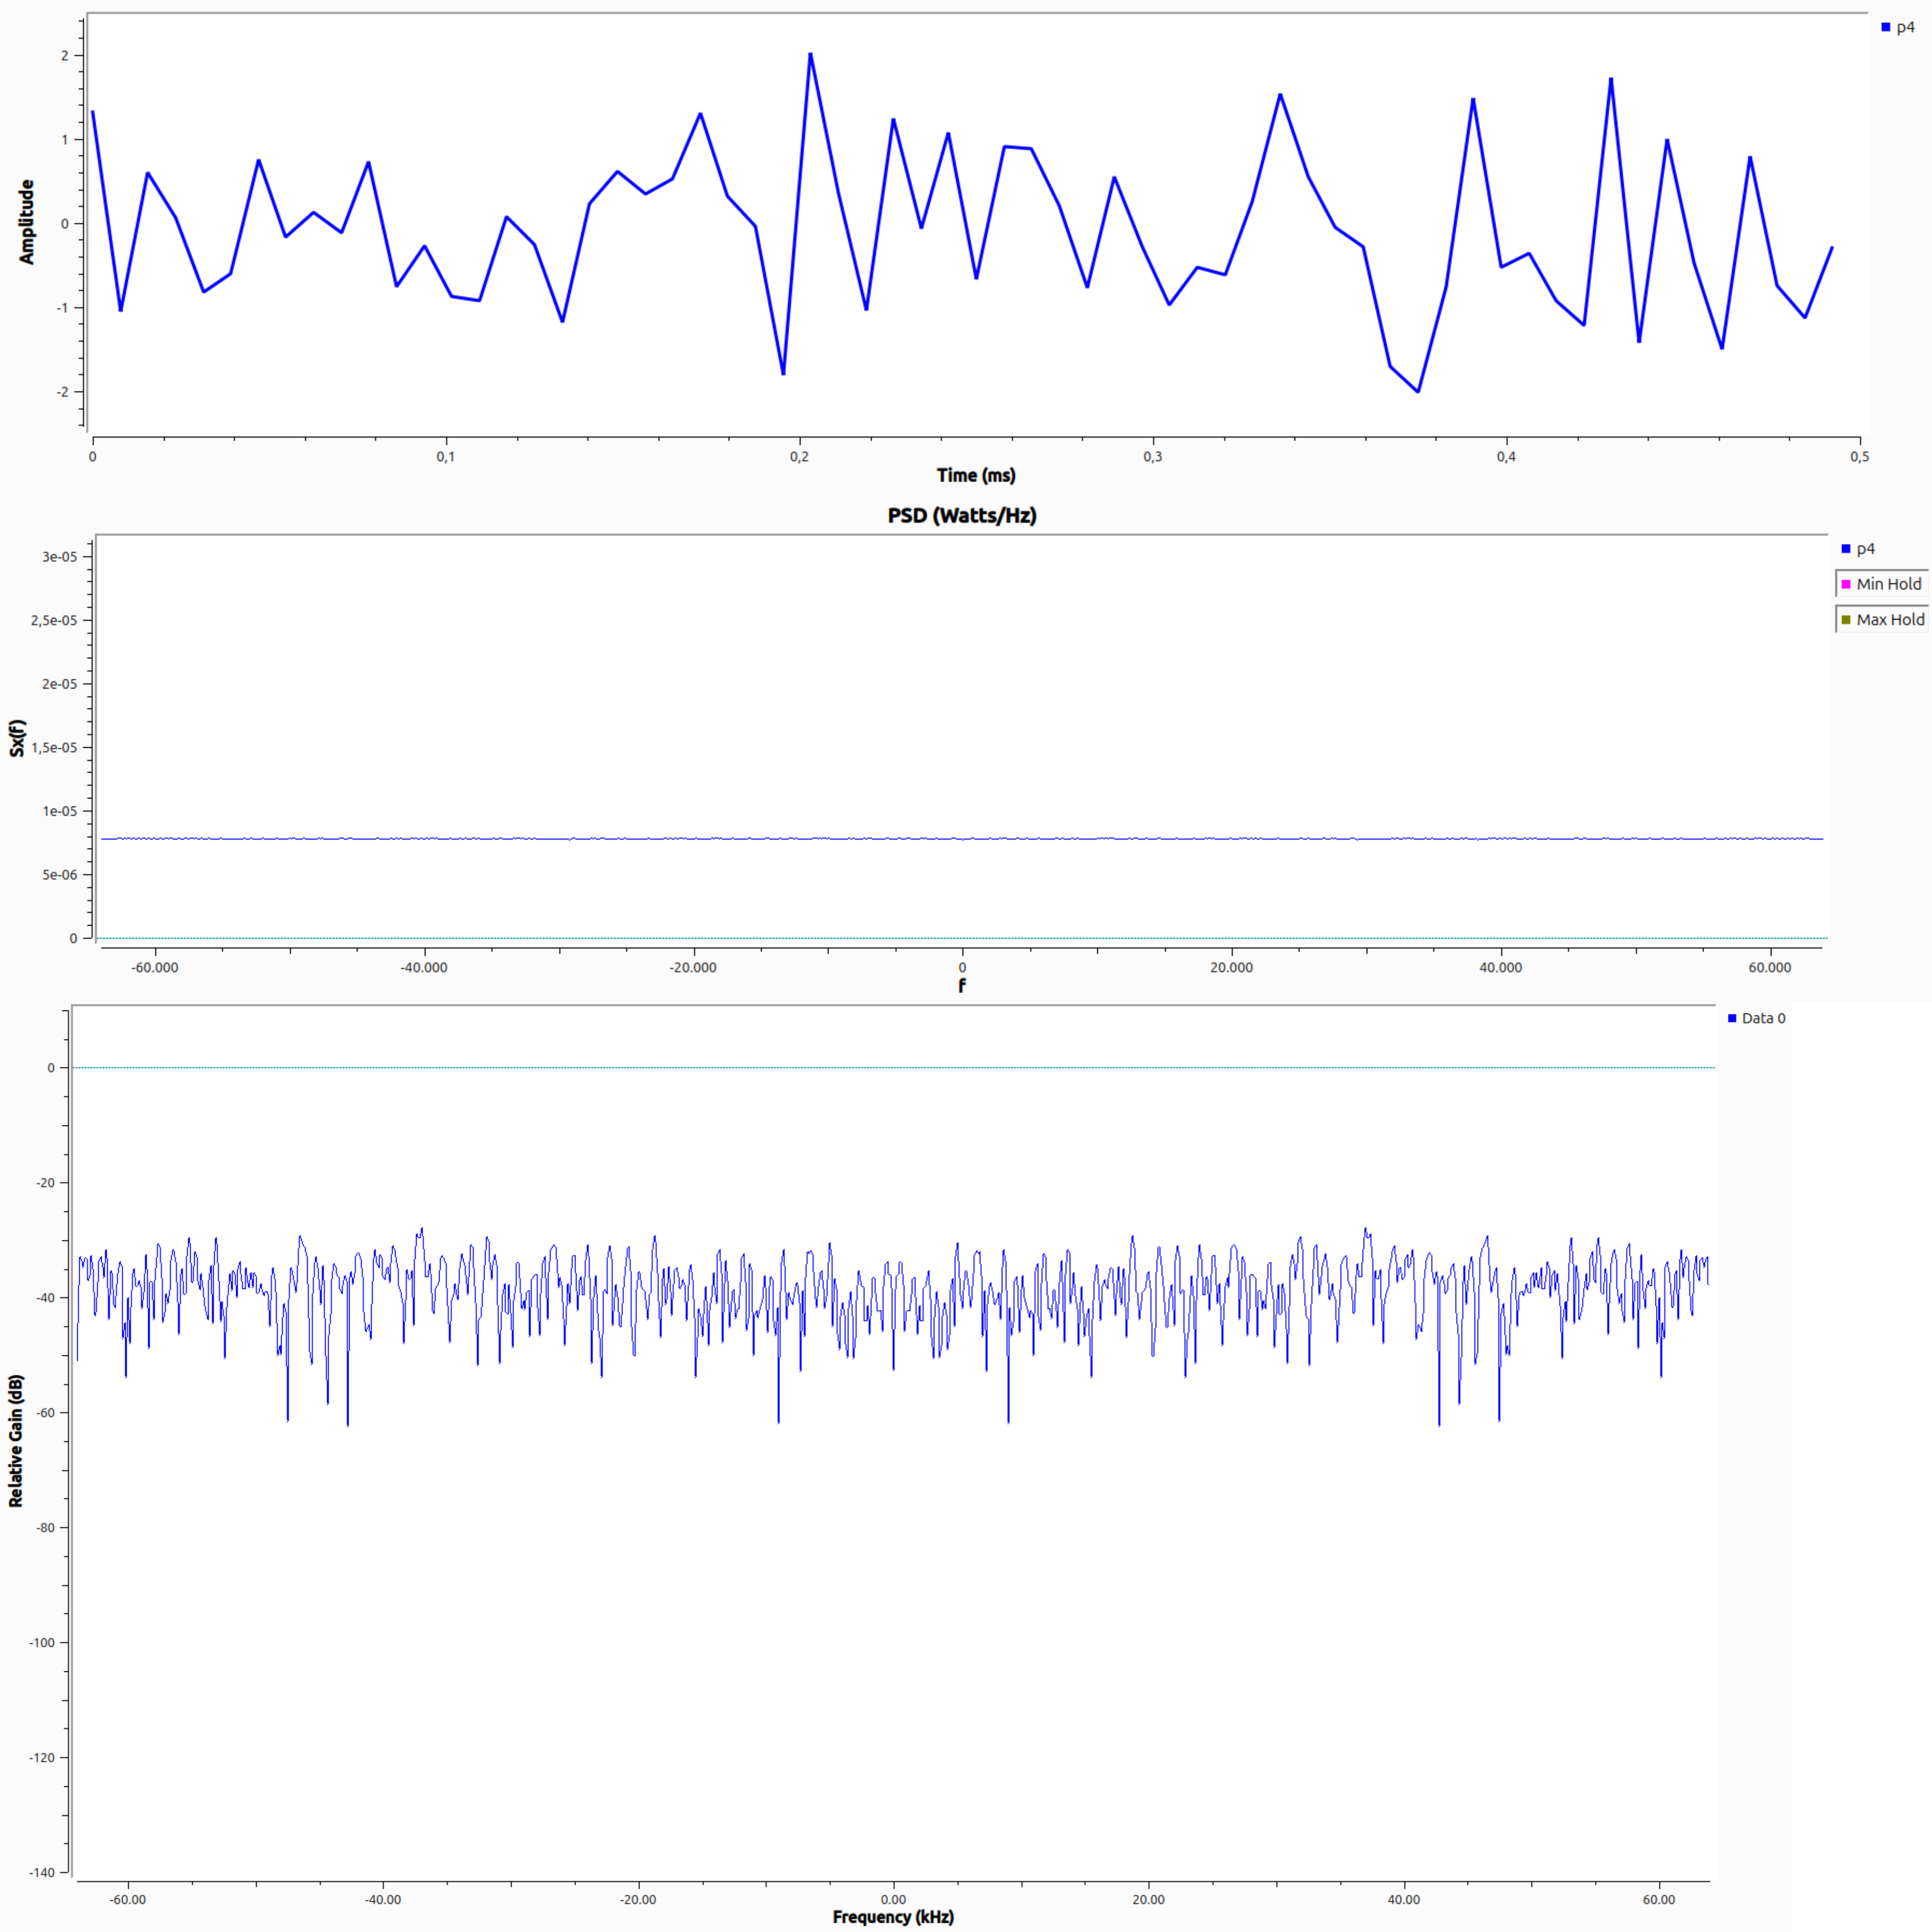
\includegraphics[width=0.6\linewidth]{1788670039509_image.png}
    \caption{Ruido blanco gaussiano (p5). \textbf{Arriba}: forma en el tiempo y PSD (Watts/Hz). \textbf{Abajo}: PSD en dB sobre una banda de análisis más amplia.}
    \label{fig:ruido}
\end{figure}

A diferencia de las señales binarias, la amplitud del ruido no estuvo acotada a $\pm 1$ (en el panel superior se observaron picos de hasta $\pm 2$) y su PSD se mantuvo aproximadamente constante en toda la banda mostrada, tanto en escala lineal (eje $\pm60$ kHz) como en dB (banda más amplia), sin lóbulos ni nulos apreciables, lo cual fue consistente con la definición teórica de ruido blanco \cite{ortega2019comunicaciones}. Sin embargo, el ancho de banda infinito del ruido blanco ideal no pudo observarse en GNU Radio, ya que la frecuencia de muestreo $f_s$ limitó el espectro representable al rango $[-f_s/2, f_s/2]$; lo que se observó fue, en realidad, ruido blanco limitado en banda por el propio muestreo.

\subsection{Señal binaria a partir de una imagen (rana.jpg)}

\begin{figure}[h]
    \centering
    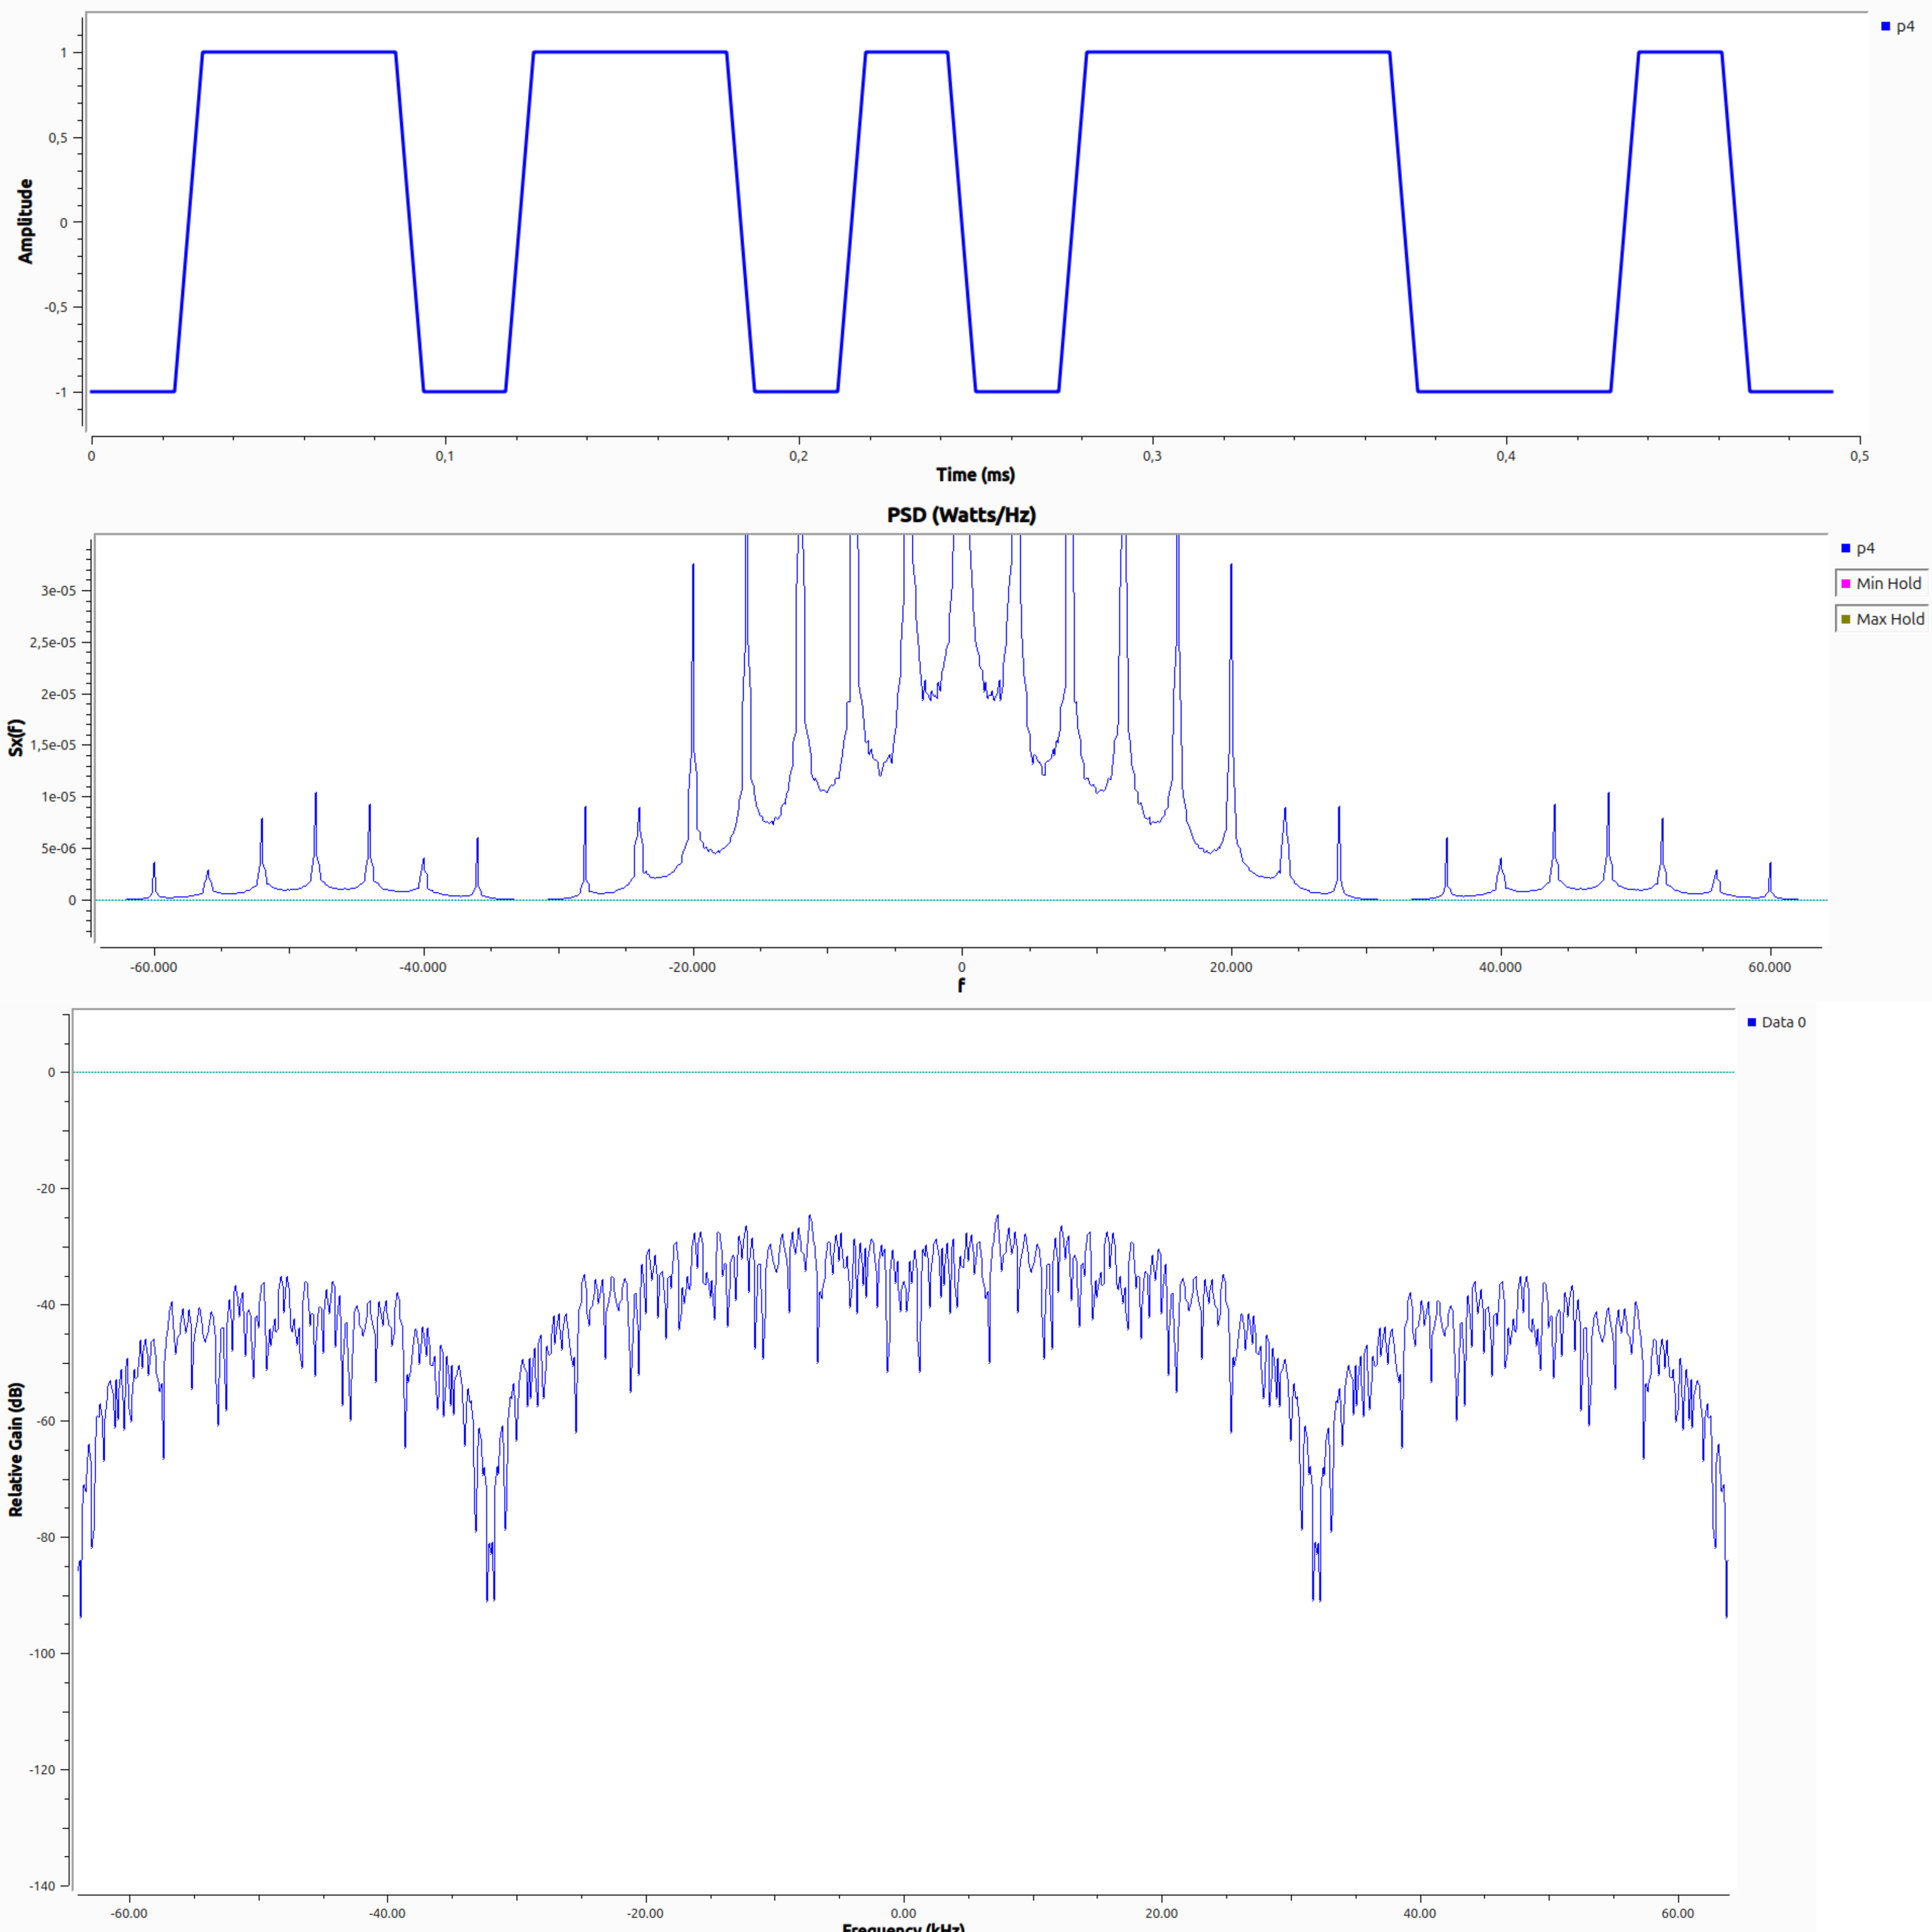
\includegraphics[width=0.48\linewidth]{1788672884845_image.png}
    \hfill
    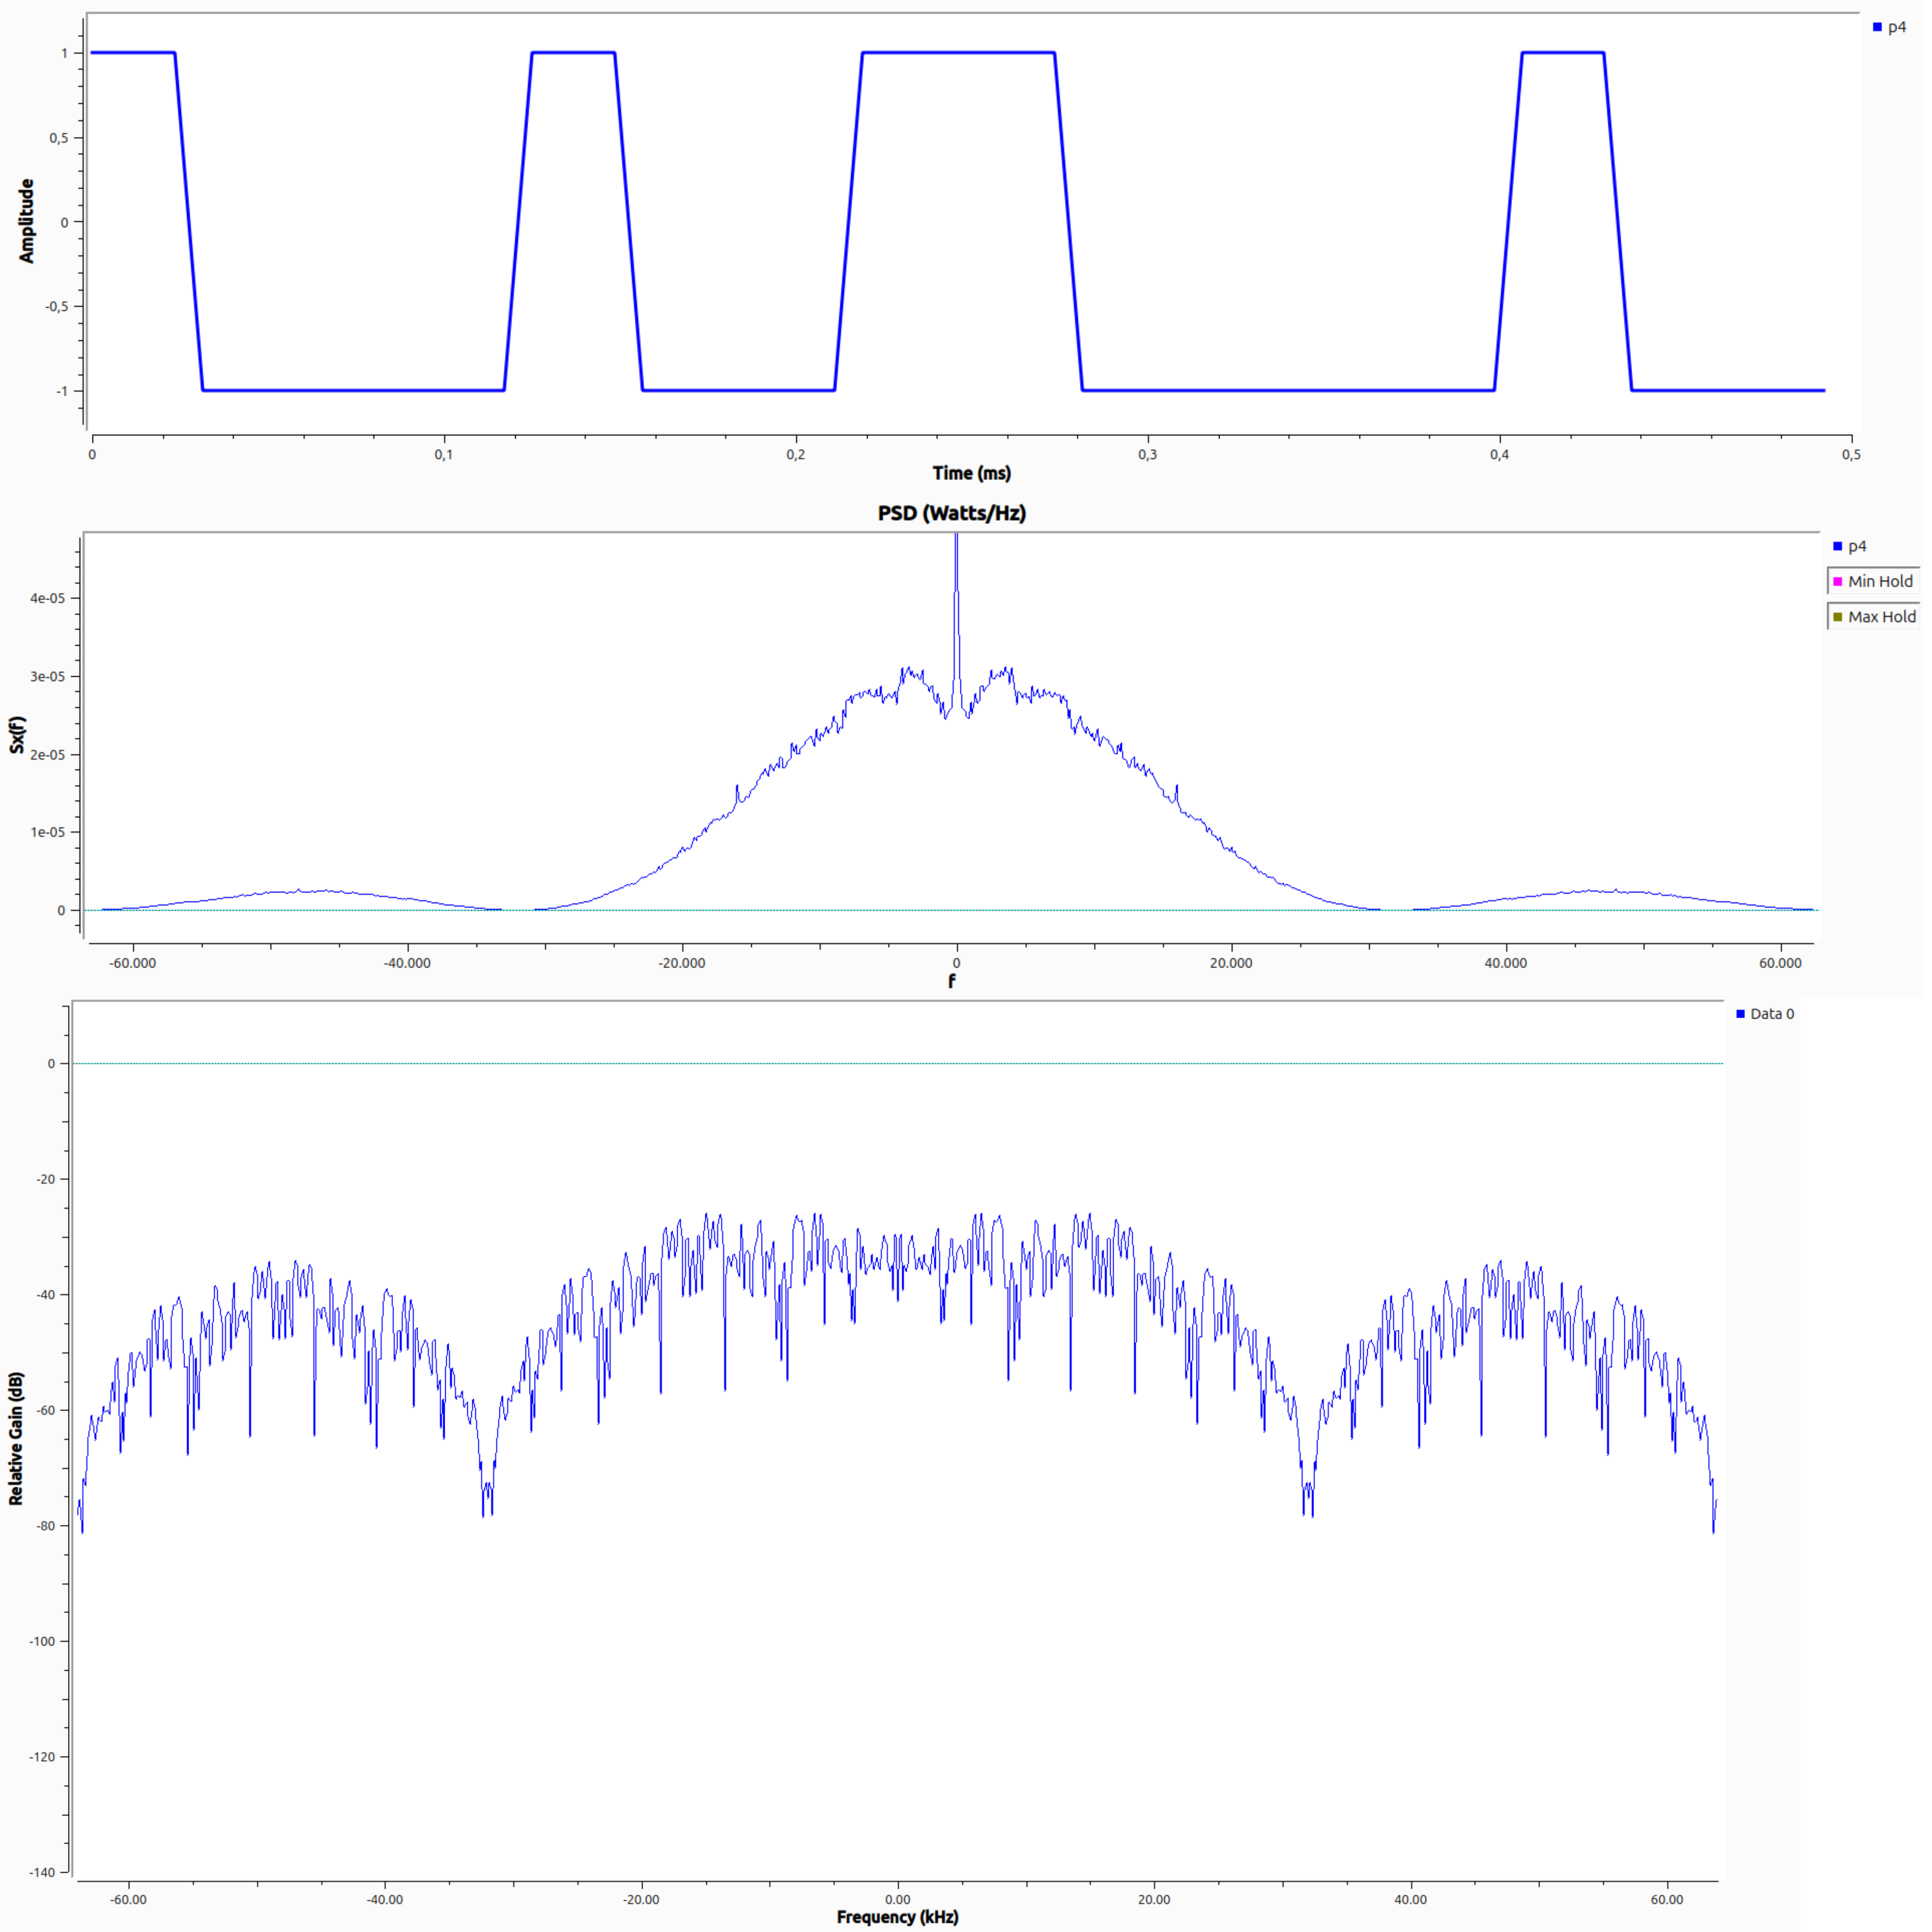
\includegraphics[width=0.48\linewidth]{1788670106061_image.png}
    \caption{\textbf{Izquierda}: Señal binaria a partir de \texttt{sonido.wav} \cite{ortega2021sonido} con $Sps=4$. Arriba: forma en el tiempo en p4. Abajo: PSD (Watts/Hz). 
    \textbf{Derecha}: Señal binaria a partir de \texttt{rana.jpg} \cite{ortega2021rana}. Arriba: tiempo y PSD (Watts/Hz). Abajo: PSD en dB.}
    \label{fig:audio_imagen}
\end{figure}
En el panel izquierdo superior de la Figura~\ref{fig:audio_imagen} la forma en el tiempo fue visualmente similar a la de la Figura~\ref{fig:sps4} (pulsos rectangulares limpios), ya que se usó el mismo $Sps=4$. En el panel intermedio (PSD lineal), la envolvente general conservó la forma $\text{sinc}^2$, pero se distinguió un pico espectral discreto —mucho más alto y angosto que el resto del lóbulo principal— exactamente en $f=0$ Hz. Esto ocurrió porque los bytes de una imagen no son estadísticamente independientes como los de un \emph{Random Source}: existían patrones repetitivos (filas de píxeles similares y encabezados del archivo) que introducían periodicidades en la secuencia de bits y, por tanto, generaban una media no nula o componente DC, la cual se manifestó como ese impulso superpuesto a la envolvente. El panel inferior (dB) mostró la misma envolvente con nulos periódicos, cubierta por el rizado propio de la estimación por periodograma \cite{tijaro2025timeaverages}.

La media teórica era cero, pero se obtuvieron $-0.061851$ y $0.000488$, fluctuación esperada por el promedio sobre una ventana finita y despreciable frente a la Potencia Promedio $=1.0$.

\subsection{Señal binaria a partir de un archivo de audio (sonido.wav)}


En el dominio del tiempo (Figura~\ref{fig:audio_imagen}, panel superior derecho) la señal conservó la forma bipolar rectangular esperada, pero con anchos de pulso irregulares: en lugar de una secuencia estadísticamente independiente de símbolos, se observaron tramos con varios símbolos consecutivos del mismo signo, reflejo de la correlación entre bytes vecinos propia de una señal de audio, donde muestras consecutivas de una forma de onda continua tienden a compartir bits en común.

Esta correlación se manifestó con más fuerza en la PSD que en el caso de la imagen. En el panel inferior (escala lineal, eje $\pm60$ kHz) se observó un peine de líneas espectrales mucho más denso y con picos más pronunciados que los obtenidos con \texttt{rana.jpg}, concentrados principalmente entre $\pm 5$ y $\pm 20$ kHz, con líneas adicionales de menor amplitud que se extendían hasta cerca de $\pm60$ kHz. Esto ocurrió porque una señal de audio real suele contener componentes tonales o cuasi-periódicas (p. ej. una nota sostenida o un patrón rítmico), lo que generó una periodicidad mucho más marcada en la secuencia de bits que la simple repetición de encabezados o filas similares de una imagen.

Al observar la PSD en escala logarítmica se distinguió con claridad la envolvente continua tipo $\text{sinc}^2$ por debajo del peine de líneas: el lóbulo principal se extendió hasta un primer nulo cercano a $\pm 32$ kHz y un segundo nulo cercano a $\pm 64$ kHz, coincidiendo con el $BW$ teórico de 64 kHz calculado para $Sps=4$ en la Tabla~\ref{tab:sps}. Esto confirmó que, independientemente de si los bits provenían de una fuente aleatoria, una imagen o un audio, la envolvente de la PSD estaba determinada por la forma del pulso y por $Sps$ (a través de $R_b$); lo que cambiaba con el tipo de fuente era únicamente la presencia y la intensidad de las líneas espectrales discretas superpuestas a esa envolvente, las cuales fueron más numerosas y de mayor amplitud cuanto mayor era la periodicidad interna de los datos de origen (audio > imagen > fuente aleatoria).

















\subsection*{Preguntas de control}

Las respuestas completas a todas las preguntas de control se encuentran en el
\href{https://github.com/J202R/2026_2_ComII_A1_A1E/blob/8561d6605cb175f4b1f52bd0fa1fc54990ee867e/Pr%C3%A1ctica_2/respuestas%20a%20preguntas/preguntas.pdf}
{\textbf{documento de respuestas disponible en el repositorio}}.




El bloque \textit{Throttle} controla la velocidad de procesamiento en una simulación de GNU Radio, mientras que con hardware SDR el flujo de muestras es controlado por el dispositivo. Para una señal unipolar (0,1), la PSD presenta una componente DC  a su valor medio no nulo; en cambio, una señal bipolar balanceada (-1,+1) tiene valor medio cercano a cero y reduce dicha componente.

La relación fundamental del sistema es
\[
R_b=\frac{f_s}{Sps},
\]
por lo que al aumentar \(Sps\) disminuye la tasa de bits y se reduce el ancho de banda principal. Para la señal rectangular NRZ, el primer nulo aparece aproximadamente en \(R_b\), de modo que el ancho de banda entre primeros nulos es \(BW=2R_b\). El espectro observado está limitado por \(f_s\), es decir, por el intervalo \([-f_s/2,f_s/2]\). La resolución de la PSD depende además del tamaño de la FFT, según
\[
\Delta f=\frac{f_s}{N}.
\]

El bloque \textit{Unpack K Bits} transforma cada elemento de entrada en \(K\) bits, aumentando la tasa de muestras, mientras que \textit{Char to Float} solamente cambia el tipo de dato y no modifica la frecuencia de muestreo. Cuando \(Sps=1\), cada bit ocupa una sola muestra y una secuencia bipolar aleatoria presenta una PSD aproximadamente plana dentro del ancho de banda observado, comportamiento semejante al ruido blanco.

Finalmente, diferentes formas de señal pueden obtenerse modificando el filtro y la portadora: RZ y Manchester se generan modificando la forma temporal de cada símbolo; OOK y ASK representan la información mediante variaciones de amplitud de una portadora, mientras que BPSK utiliza los niveles bipolares para producir cambios de fase de \(180^\circ\). En todos los casos, la forma del pulso determina la envolvente espectral, mientras que la secuencia de datos determina las componentes adicionales de la PSD.


\section{Conclusiones}

Los resultados verifican la relación teórica $R_b = f_s/Sps$ de la Tabla~\ref{tab:sps}: en la Figura~\ref{fig:sps4} el primer nulo se ubica cerca de $32$ kHz, próximo al $R_b=32$ kHz teórico, y al comparar con las Figuras~\ref{fig:sps8} y~\ref{fig:sps16} el lóbulo principal se angosta a medida que aumenta \emph{Sps}, confirmando la relación inversa entre muestras por símbolo y ancho de banda ocupado.

El ruido blanco gaussiano (Figura~\ref{fig:ruido}) no presenta lóbulos ni nulos y su PSD se mantiene aproximadamente constante, consistente con su ancho de banda teóricamente infinito; lo observado es, en realidad, ruido limitado en banda por $f_s=128$ kHz.

Con bits de una imagen (\texttt{rana.jpg} \cite{ortega2021rana} , Figura~\ref{fig:audio_imagen}) y de audio (\texttt{sonido.wav}  \cite{ortega2021sonido}, Figura~\ref{fig:audio_imagen}), la envolvente $\text{sinc}^2$ se conserva, y en el audio los nulos cercanos a $\pm32$ kHz y $\pm64$ kHz coinciden con el $BW$ teórico de $64$ kHz para $Sps=4$. Esto confirma que la envolvente depende de la forma del pulso y de $Sps$, no del origen de los bits. Lo que sí cambia es la presencia de componentes discretas superpuestas: un impulso en $f=0$ para la imagen, y un peine de líneas más denso para el audio, reflejo de la mayor correlación interna de una señal de audio real.

En conjunto, estos resultados sustentan la relación inversa entre $Sps$ y el ancho de banda ocupado, y la independencia de la envolvente espectral respecto al origen estadístico de los bits.














\nocite{*}

\bibliographystyle{IEEEtran}
\bibliography{bibliografia}

\end{document}